%----------------------------------------------------------------------------------------------------
\section{Analysis}

The analysis method is similar to the previously published ones~\cite{epl101-el,prl111}. In particular, each diagonal is analysed
separately. However, a different normalisation
approach is used (Section~\ref{sec:normalisation}) that makes all 
$t$-independent scaling factors irrelevant.

The analysis is presented in two main blocks. Section~\ref{sec:event anal} covers all aspects related to the reconstruction of a single event.
Section~\ref{sec:diff cs} describes the steps of transforming a raw $t$-distribution into the differential cross-section. The $t$-distributions for the two diagonals are analysed separately. After comparison (Section~\ref{sec:cross checks}) they are finally merged (Section~\ref{sec:final data merging}).

%----------------------------------------------------------------------------------------------------

\subsection{Event Analysis}
\label{sec:event anal}

Event kinematics are determined from coordinates of track hits in the RPs after proper alignment (see Section~\ref{sec:alignment}), using the LHC optics (see Section~\ref{sec:optics}).


%------------------------------

\subsubsection{Kinematics Reconstruction}
\label{sec:kinematics}

The scattering angles and vertex position are first determined for each proton (i.e.~from each arm) separately by inverting the proton transport, Eq.~(\ref{eq:prot trans}), assuming $\xi = 0$. The following formulae optimise the robustness against optics imperfections:
\begin{equation}
\label{eq:kin 1a}
	\begin{aligned}
		\theta_x^{*L,R} &= {v_x^{\rm N} x^{\rm F} - v_x^{\rm F} x^{\rm N}\over v_x^{\rm N} L_x^{\rm F} - v_x^{\rm F} L_x^{\rm N}}\ ,\qquad
		\theta_y^{*L,R} = {1\over 2} \left( {y^{\rm N}\over L_y^{\rm N}} + {y^{\rm F}\over L_y^{\rm F}} \right)\ ,\\
		x^{*L,R} &= {L_x^{\rm N} x^{\rm F} - L_x^{\rm F} x^{\rm N}\over L_x^{\rm N} v_x^{\rm F} - L_x^{\rm F} v_x^{\rm N}}\ , \\
	\end{aligned}
\end{equation}
where the N and F superscripts refer to the near and far units, L and R to the 
left and right arm, respectively. This one-arm reconstruction is used for tagging elastic events, where the left and right arm protons are compared.

Once an event is selected, the information from both arms is merged yielding better angular resolution:
\begin{equation}
\label{eq:kin 2a}
\theta_x^* = {\theta_x^{*\rm L} + \theta_x^{*\rm R} \over 2}\ ,\quad \theta_y^* = {\theta_y^{*\rm L} + \theta_y^{*\rm R} \over 2}\ .
\end{equation}
Eventually, the full scattering angle, $\theta^*$, and four-momentum transfer squared, $t$, are calculated as

\begin{equation}
\label{eq:th t}
\theta^* = \sqrt{{\theta_x^*}^2 + {\theta_y^*}^2}\ ,\quad t = - p^2 ({\theta_x^*}^2 + {\theta_y^*}^2)\ ,
\end{equation}
where $p$ denotes the beam momentum.

%------------------------------

\subsubsection{Alignment}
\label{sec:alignment}

The standard three-step procedure \cite{totem-ijmp} has been applied: beam-based alignment prior to the run (as for LHC collimators) followed by two off-line methods. First, track-based alignment for relative positions among RPs, and second, alignment with elastic events for absolute position with respect to the beam. The final uncertainties per unit (common for top and bottom RPs) are: $2\un{\mu m}$ (horizontal shift), $100\un{\mu m}$ (vertical shift) and $0.2\un{mrad}$ (rotation about the beam axis). Propagated to the scattering angles, Eq.~(\ref{eq:kin 2a}), the shifts lead to uncertainties of $0.8\un{\mu rad}$ (horizontal) and $0.2\un{\mu rad}$ (vertical). The error of the RP rotations would bias the reconstructed horizontal scattering angle:
\begin{equation}
\label{eq:alig rot bias}
\theta_x^* \rightarrow \theta_x^* + c \theta_y^*\ ,
\end{equation}
where the proportionality constant $c$ has a standard deviation of $0.02$.



%------------------------------

\subsubsection{Optics}
\label{sec:optics}
%
In order to reduce the impact of imperfect optics knowledge, the optics matching technique \cite{totem-optics} has been applied. This method uses various RP observables to determine fine corrections to the optical functions presented in Eq.~(\ref{eq:prot trans}).

The residual errors induce a bias in the reconstructed scattering angles:
\begin{equation}
\label{eq:opt bias}
\theta_x^* \rightarrow (1 + d_x)\, \theta_x^*\ ,\quad
\theta_y^* \rightarrow (1 + d_y)\, \theta_y^*\ .
\end{equation}
For the two-arm reconstruction, Eq.~(\ref{eq:kin 2a}), the biases $d_x$ and $d_y$ have uncertainties of $0.21\un{\%}$ and $0.25\un{\%}$, respectively, and correlation factor of $-0.70$. These estimates include the effects of magnet harmonics.
%
%
% Mario's version
\iffalse
For evaluating the impact on the $t$-distribution, it is convenient to decompose the correlated biases $d_x$ and $d_y$ in two statistically independent modes, $\mathbf{\tilde{d}_{1}}$ and $\mathbf{\tilde{d}_{2}}$, obtained by diagonalising the covariance matrix:
\begin{equation}
\label{eq:opt bias modes}
\begin{pmatrix} d_x\cr d_y \end{pmatrix} =
	\eta_1 \mathbf{\tilde{d}_{1}} 
	+ \eta_2 \mathbf{\tilde{d}_{2}} \ ,
\end{equation}
where $\mathbf{\tilde{d}_{1}} = \begin{pmatrix} -0.182\un{\%} \cr +0.235\un{\%} \end{pmatrix}$ and $\mathbf{\tilde{d}_{1}} = \begin{pmatrix} -0.096\un{\%} \cr -0.074\un{\%} \end{pmatrix}$ are orthogonal, and the factors $\eta_{1,2}$ have unit variance.
\fi
%
%
For evaluating the impact on the $t$-distribution, it is convenient to decompose the correlated biases $d_x$ and $d_y$ into eigenvectors of the covariance matrix:
\begin{equation}
\label{eq:opt bias modes}
\begin{pmatrix} d_x\cr d_y \end{pmatrix} =
	\eta_1 \underbrace{\begin{pmatrix} -0.182\un{\%} \cr +0.235\un{\%} \end{pmatrix}}_{\rm mode\ 1}
	+ \eta_2 \underbrace{\begin{pmatrix} -0.096\un{\%} \cr -0.074\un{\%} \end{pmatrix}}_{\rm mode\ 2}
\end{equation}
normalised such that the factors $\eta_{1,2}$ have unit variance.

%------------------------------

\subsubsection{Resolution}
\label{sec:resolution}

Statistical fluctuations in the reconstructed scattering angles are caused by the beam divergence and, in the horizontal projection (due to small $L_x$), also by the sensor resolution. They are studied by comparing the scattering angles reconstructed from the two arms, in particular through differences $\theta_{x,y}^{*R} - \theta_{x,y}^{*L}$ as illustrated in Figure \ref{fig:beam divergence}. The distributions exhibit small deviations from Gaussian shape which decrease with time.

Since in good approximation the fluctuations are independent in each arm, the angular resolution for the two-arm reconstruction, Eq.~(\ref{eq:kin 2a}), is given by half of the standard deviation of the $\theta_{x,y}^{*R} - \theta_{x,y}^{*L}$ distributions. As shown in Figure~\ref{fig:resolutions}, the resolution deteriorates slightly with time, which can be expected mainly due to the emittance growth. The small difference in $\theta_x^*$ resolution between the diagonals can be attributed to different RPs, each with slightly different spatial resolution, being involved in the two diagonals.

Measurements of beam emittances~\cite{op-elog} show that the vertical beam divergences of the two beams are equal with a tolerance of about $15\un{\%}$. Exploiting this equality, one can de-convolute the distribution of $\theta_y^{*R} - \theta_y^{*L}$ in order to obtain the beam-divergence distribution, used e.g.~for acceptance corrections (see Section~\ref{sec:acc corr}).

\begin{figure}
\begin{center}
% Do not scale the graphics - fonts have been adjusted to match with figure caption.
% If needed, ask for a different size at jan.kaspar@cern.ch.
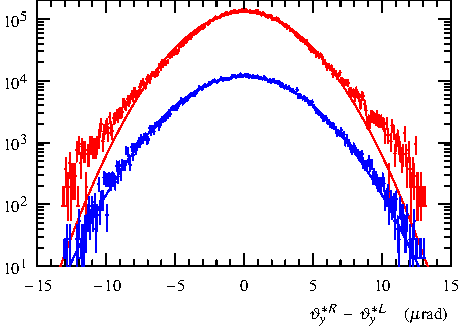
\includegraphics{fig/beam_divergence_fits.pdf}
\vskip-4mm
\caption{%
Difference between vertical scattering angles reconstructed in the right and left arm, for the diagonal 45 bottom - 56 top. Red: data from run start ($0.5$ to $1.5\un{h}$ from the beginning of the run). Blue: data from run end ($10.5$ to $11.5\un{h}$), scaled by $0.1$. The solid lines represent Gaussian fits.
}
\label{fig:beam divergence}
\end{center}
\end{figure}



\begin{figure}
\begin{center}
% Do not scale the graphics - fonts have been adjusted to match with figure caption.
% If needed, ask for a different size at jan.kaspar@cern.ch.
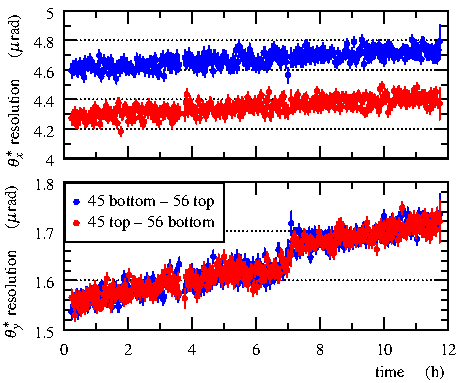
\includegraphics{fig/resolutions_vs_time.pdf}
\vskip-4mm
\caption{%
Angular resolution for the two-arm reconstruction, Eq.~(\ref{eq:kin 2a}), as a function of time (from the beginning of the run). The step in $\theta_y^*$ resolution around $7\un{h}$ is due to inclusion of another proton bunch with a larger vertical emittance.
}
\label{fig:resolutions}
\end{center}
\end{figure}




%----------------------------------------------------------------------------------------------------

\subsection{Differential Cross-Section}
\label{sec:diff cs}

For a given $t$ bin, the differential cross-section is evaluated by selecting and counting elastic events:
\begin{equation}
{\d\sigma\over \d t}(\hbox{bin}) =
	{\cal N}\, {\cal U}({\rm bin})\, {\cal B}\ 
	{\sum\limits_{t \in \hbox{bin}} {\cal A}(\theta^*, \theta_y^*)\, {\cal E}(\theta_y^*)\over \Delta t}\ ,
\end{equation}
where $\Delta t$ is the width of the bin, ${\cal N}$ is a normalisation factor, 
and the other symbols stand for various correction factors:
${\cal U}$ for unfolding of resolution effects, ${\cal B}$ for background subtraction, ${\cal A}$ for acceptance correction and ${\cal E}$ for detection and reconstruction efficiency.

%------------------------------

\subsubsection{Event Tagging}
\label{sec:tagging}

The cuts used to select elastic events are summarised in Table \ref{tab:cuts}. Cuts 1 and 2 require the reconstructed-track collinearity between the left and right arm. Cuts 3 and 4 control the elasticity -- if a proton loses momentum, the vertical position-angle correlation at the RPs is lost. Cut 5 ensures that the two protons come from the same vertex (horizontally). The correlation plots corresponding to these cuts are shown in Figure~\ref{fig:cuts}.

Monte-Carlo simulation suggests that applying all the five cuts at $3\un{\sigma}$ level would lead to a loss of about $2\un{\%}$ of elastic events. Setting the thresholds to $4\un{\sigma}$ yields a tolerable loss of about $0.07\un{\%}$ and therefore the cuts are applied at the $4\un{\sigma}$ level.
% 2sigma: 76%, 3sigma: 98.02%, 4sigma: 99.93%, 5sigma: 99.999%

The tagging efficiency is studied experimentally by applying the cuts also at the $5\un{\sigma}$ level. This selection yields about $0.5\un{\%}$ more events in every $t$ bin -- thus the inefficiency is irrelevant for this analysis.


\begin{table}
\caption{The elastic selection cuts. The superscripts R and L refer to the right and left arm, N and F correspond to the near and far units, respectively. The constant $\alpha = L_y^{\rm F} / L_y^{\rm N} - 1 \approx 0.11$. The right-most column gives a typical RMS of the cut distribution.
}
\label{tab:cuts}
\begin{center}
\vskip-3mm
\begin{tabular}{ccc}\hline\hline
discriminator & cut quantity & RMS ($\equiv 1\sigma$)\cr\hline
1 & $\theta_x^{*\rm R} - \theta_x^{*\rm L}$				& $9.5\un{\mu rad}$	\cr
2 & $\theta_y^{*\rm R} - \theta_y^{*\rm L}$				& $3.3\un{\mu rad}$	\cr
3 & $\alpha\,y^{\rm R,N} - (y^{\rm R,F} - y^{\rm R,N})$	& $18\un{\mu m}$	\cr
4 & $\alpha\,y^{\rm L,N} - (y^{\rm L,F} - y^{\rm L,N})$	& $18\un{\mu m}$	\cr
5 & $x^{*\rm R} - x^{*\rm L}$							& $8.5\un{\mu m}$ 	\cr\hline\hline
\end{tabular}
\end{center}
\end{table}

\begin{figure*}
\begin{center}
% Do not scale the graphics - fonts have been adjusted to match with figure caption.
% If needed, ask for a different size at jan.kaspar@cern.ch.
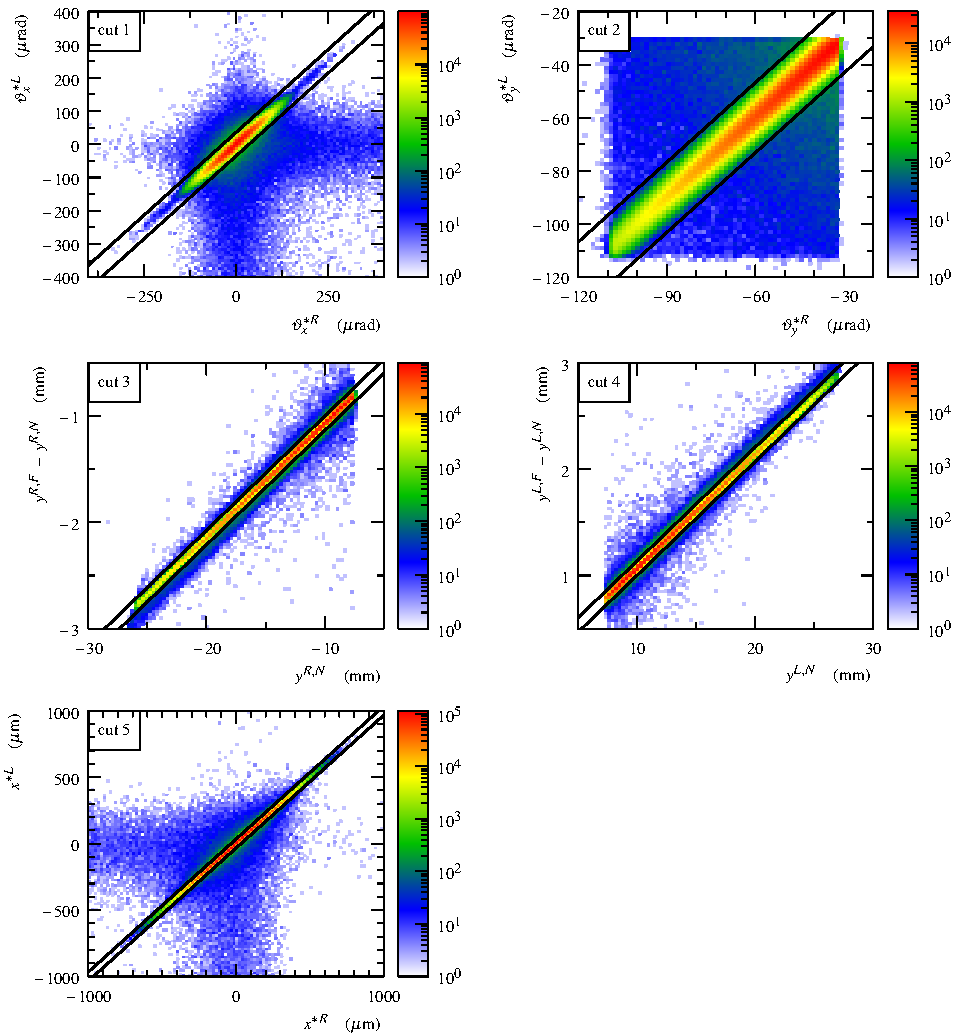
\includegraphics{fig/cuts.pdf}
\caption{%
Correlation plots for the event selection cuts summarised in Table~\ref{tab:cuts}, using all events with diagonal topology 45 top -- 56 bottom. The black solid lines delimit the signal ($\pm 4\un{\sigma}$) region.
}
\label{fig:cuts}
\end{center}
\end{figure*}


%------------------------------

\subsubsection{Background}
\label{sec:background}

Expectable background (i.e.~non-elastic events passing the tagging cuts) may come from central diffraction as well as pile-up of single diffraction and/or beam-halo protons. The background rate is studied by plotting the discriminators from Table~\ref{tab:cuts} under various cut combinations, see an example in Figure~\ref{fig:background}. While the central part (signal) remains essentially constant, the tails (background) are strongly suppressed with increasing number of cuts applied. This interpretation is further supported by the discriminator distributions from anti-diagonal RP configurations, see the dotted curves in the figure. While these top -- top or bottom -- bottom configurations cannot contain any elastic signal, they are likely to have a similar share of events causing background to the presented analysis. And indeed, the figure shows a good agreement at the distribution tails. Integrating the anti-diagonal curve over the signal region (see the dashed lines in the figure) yields a background estimate of $1 - {\cal B} < 10^{-4}$.
%, independent of whether discriminator 1, 2 or 5 is used.
% anyway irrelevant due to the normalisation approach


\begin{figure}
\begin{center}
% Do not scale the graphics - fonts have been adjusted to match with figure caption.
% If needed, ask for a different size at jan.kaspar@cern.ch.
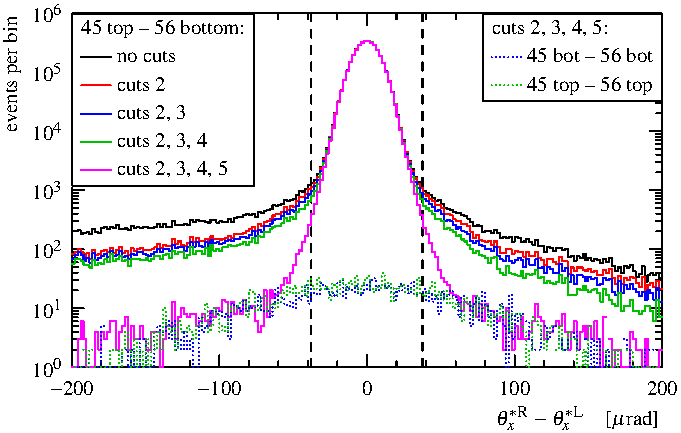
\includegraphics{fig/cut_distributions.pdf}
\caption{%
Distributions of discriminator 1, i.e. the difference between the horizontal scattering angle reconstructed from the right and the left arm. Solid curves: data from diagonal 45 top -- 56 bottom, the different colours correspond to various combinations of the selection cuts (see numbering in Table~\ref{tab:cuts}). Dotted curves: data from anti-diagonal RP configurations, obtained by inverting track coordinates in the left arm. The vertical dashed lines represent the boundaries of the signal region ($\pm 4\un{\sigma}$).
}
\label{fig:background}
\end{center}
\end{figure}

%-------------------------

\subsubsection{Acceptance Correction}
\label{sec:acc corr}

Two proton detection limitations have been identified: detector coverage (mostly at the edge facing the beam, i.e. relevant for small $|\theta_y^*|$) and LHC apertures ($|\theta_y^*| \approx 100\un{\mu rad}$). The correction accounting for these limitations includes two contributions -- a geometrical correction ${\cal A}_{\rm geom}$ reflecting the fraction of the phase space within the acceptance and a component ${\cal A}_{\rm fluct}$ correcting for fluctuations around the acceptance limitations (cuts in $\theta_y^*$):
\begin{equation}
{\cal A}(\theta^*, \theta_y^*) = {\cal A}_{\rm geom}(\theta^*)\ {\cal A}_{\rm fluct}(\theta_y^*)\ .
\end{equation}

The calculation of the geometrical correction ${\cal A}_{\rm geom}$ is based on the azimuthal symmetry of elastic scattering, experimentally verified for the data within acceptance. As shown in Figure \ref{fig:acceptance principle}, for a given value of $\theta^*$ the correction is given by:
\begin{equation}
\label{eq:acc geom}
{\cal A_{\rm geom}}(\theta^*) = {
	\hbox{full arc length}\over 
	\hbox{arc length within acceptance}
} \ .
\end{equation}


\begin{figure}
\begin{center}
% Do not scale the graphics - fonts have been adjusted to match with figure caption.
% If needed, ask for a different size at jan.kaspar@cern.ch.
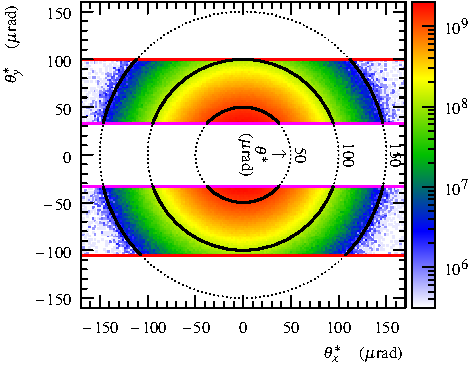
\includegraphics{fig/acc_corr_phi_lab.pdf}
\vskip-3mm
\caption{%
Distribution of scattering angle projections $\theta_y^*$ vs.~$\theta_x^*$. The upper (lower) part comes from the diagonal 45 bottom -- 56 top (45 top -- 56 bottom). The red horizontal lines represent cuts due to the LHC apertures, the magenta horizontal lines cuts due to the sensor edges. The dotted circles show contours of constant scattering angle $\theta^*$ as indicated in the middle of the plot. The parts of the contours within acceptance are emphasized in thick black.
}
\label{fig:acceptance principle}
\end{center}
\end{figure}


The correction ${\cal A}_{\rm fluct}$ is calculated analytically from the probability that any of the two elastic protons is pushed outside the acceptance due to the beam divergence. The beam divergence distribution is modelled as Gaussian with spread determined by the method described in Section~\ref{sec:resolution}. This correction contribution is only sizeable close to the acceptance limitations but is kept below $1.5$ by discarding data with larger corrections. The uncertainties are related to the resolution parameters (vertical beam divergence, left-right asymmetry and non-Gaussian shape), and all stay below $0.1\un{\%}$.


\iffalse
\begin{equation}
\label{acceptance}
{\cal A_{\rm sm}}(\theta_y^*)^{-1} = {1\over 2} \left(
	\mathop{\rm Erf} {\min(\theta_y^{*,R,max} - |\theta_y^*|, |\theta_y^*| - \theta_y^{*,L,min})\over \sigma^{1a}_{\theta_y^*}}
	- \mathop{\rm Erf} {\max(\theta_y^{*,R,min} - |\theta_y^*|, |\theta_y^*| - \theta_y^{*,L,max})\over \sigma^{1a}_{\theta_y^*}}
\right)
\end{equation}
\fi

Figure \ref{fig:acceptance result} shows an example of the acceptance correction $t$-dependence for one diagonal. Since a single diagonal cannot cover more than half of the phase space, the minimum value of the correction is $2$. As indicated in the figure, data points with too large correction (${\cal A} \gtrsim 5$) are discarded.

\begin{figure}
\begin{center}
% Do not scale the graphics - fonts have been adjusted to match with figure caption.
% If needed, ask for a different size at jan.kaspar@cern.ch.
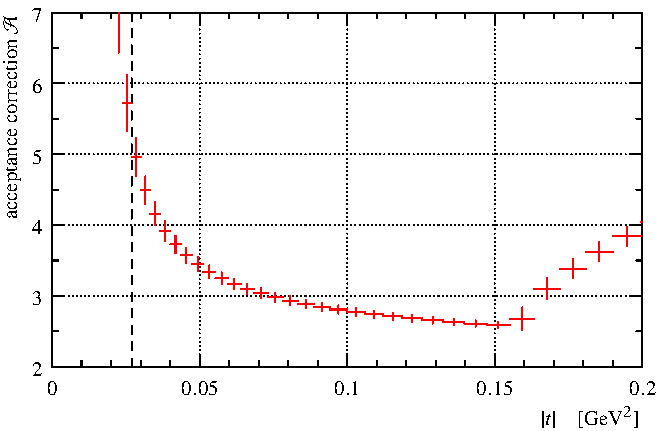
\includegraphics{fig/acc_corr_hists.pdf}
\vskip-3mm
\caption{%
Full acceptance correction, ${\cal A}$, for diagonal 45 bottom -- 56 top. The points give the mean value per bin, the error bars indicate the standard deviation. The sharp shape change at $|t|\approx 0.16\un{GeV^2}$ is caused by the LHC aperture cuts. The data left of the dashed vertical line are discarded due to excessively large acceptance correction.
}
\label{fig:acceptance result}
\end{center}
\end{figure}

%-------------------------

\subsubsection{Inefficiency Corrections}
\label{sec:ineff corr}

Since the overall normalisation is determined from another dataset (see Section~\ref{sec:normalisation}), any inefficiency correction that does not alter the $t$-distribution shape does not need to be considered in this analysis (trigger, data acquisition and pile-up inefficiency discussed in~\cite{epl101-el,prl111}). The inefficiencies left are related to inability of a RP to resolve the elastic proton track.

One such case is when a single RP cannot detect and/or reconstruct a proton track, with no correlation to other RPs. This type of inefficiency, ${\cal I}_{3/4}$, is evaluated by removing the RP from the tagging cuts (Table \ref{tab:cuts}), repeating the event selection and calculating the fraction of recovered events. A typical example is given in Figure~\ref{fig:eff 3/4}, showing that the efficiency decreases gently with the vertical scattering angle. This dependence stems from the fact that protons with larger $|\theta_y^*|$ hit the RPs further from their edge and therefore the potentially created secondary particles have more chance to induce additional signal in the sensors and thus prevent from resolving the elastic proton track.

\begin{figure}
\begin{center}
% Do not scale the graphics - fonts have been adjusted to match with figure caption.
% If needed, ask for a different size at jan.kaspar@cern.ch.
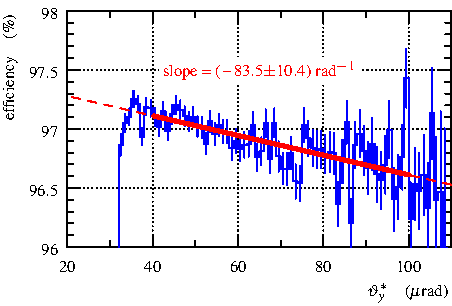
\includegraphics{fig/eff3outof4_details_fits.pdf}
\vskip-3mm
\caption{%
Single-RP uncorrelated inefficiency for the far top RP in the left arm. The rapid drop at $\theta_y^* \approx 35\un{\mu rad}$ is due to acceptance effects at the sensor edge. The red lines represent a linear fit of the efficiency dependence on the vertical scattering angle (solid) and its extrapolation to the region affected by acceptance effects (dashed).
}
\label{fig:eff 3/4}
\end{center}
\end{figure}

Another source of inefficiency are proton interactions in a near RP affecting simultaneously the far RP downstream. The contribution from these near-far correlated inefficiencies, ${\cal I}_{2/4}$, is determined by evaluating the rate of events with high track multiplicity ($\gtrsim$ 5) in both near and far RPs. Events with high track multiplicity simultaneously in a near top and near bottom RP are not counted as such a shower is likely to have started upstream from the RP station and thus unrelated to the elastic proton interacting with detectors. The outcome, ${\cal I}_{2/4} \approx 1.5\un{\%}$, compares well to Monte-Carlo simulations (e.g.~section 7.5 in \cite{hubert-thesis}).

The full correction is calculated as
\begin{equation}
\label{efficiency}
	{\cal E}(\theta_y^*) = {1\over 1 - \left( \sum\limits_{i\in \rm RPs} {\cal I}^i_{3/4}(\theta_y^*) + 2 {\cal I}_{2/4} \right) } \ .
\end{equation}
The first term in the parentheses sums the contributions from the four RPs of a diagonal and grows from about $7$ to $10\un{\%}$ from the lowest to the highest $|\theta_y^*|$. The second term amounts to about $3\un{\%}$.

%Trigger efficiency. Zero-bias data stream, events tagged as elastic, look at the trigger flag. NOT IN DS4 !!!
%For example for DS2, at $95\un{\%}$ CL, ${\cal I}_{\rm trig} < 8\cdot10^{-4}$. Anyway irrelevant.



%-------------------------

\subsubsection{Unfolding of Resolution Effects}
\label{sec:unfolding}

The correction for resolution effects has been determined by the following iterative procedure. The differential cross-section data are fitted by a smooth curve which serves as an input to a Monte-Carlo simulation using the resolution parameters determined in Section~\ref{sec:resolution}. Making a ratio between simulated histograms with and without smearing effects gives a set of per-bin correction factors. Applying them to the yet uncorrected differential cross-section yields a better estimate of the true $t$-distribution which can be used as input to the next iteration. Thanks to the good angular resolution (see Section \ref{sec:resolution}), the final correction is not large, as shown in Figure \ref{fig:unfolding}.

For the uncertainty estimate, the uncertainties of $\theta_x^*$ and $\theta_y^*$ resolutions (accommodating the full time variation) as well as fit-model dependence have been considered, the first contribution being dominant.

%2 iterations

\begin{figure}
\begin{center}
% Do not scale the graphics - fonts have been adjusted to match with figure caption.
% If needed, ask for a different size at jan.kaspar@cern.ch.
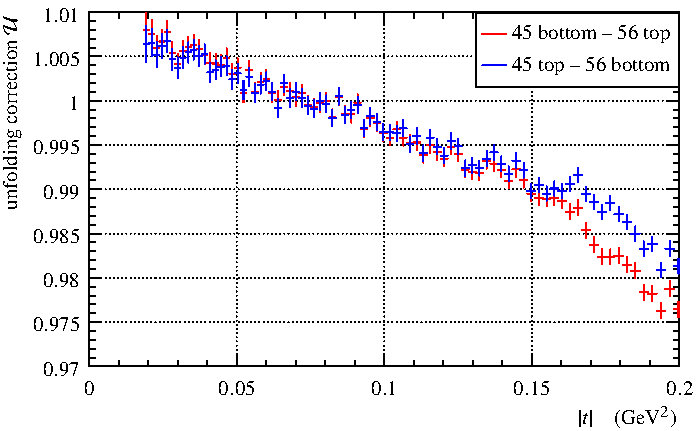
\includegraphics{fig/unfolding_correction_comparison.pdf}
\vskip-3mm
\caption{%
Unfolding correction as a function of $|t|$. The different shape for $|t| \gtrsim 0.16\un{GeV^2}$ is due to a slightly different position of the LHC aperture cut in the two diagonals.
}
\label{fig:unfolding}
\end{center}
\end{figure}

%-------------------------

\subsubsection{Normalisation}
\label{sec:normalisation}

The normalisation ${\cal N}$ is determined by requiring the same cross-section integral between $|t| = 0.027$ and $0.083\un{GeV^2}$ as for dataset 1 from \cite{prl111}, where the luminosity-independent calibration was applied. The leading uncertainty of the scaling factor $4.2\un{\%}$ comes from the luminosity-independent method.

%Leading uncertainty: lumi error from DS2 ($4.2\un{\%}$), transfer to DS4 negligible (few per-mille)


%-------------------------

\subsubsection{Binning}
\label{sec:binning}

Two binnings have been considered. The ``optimised'' option sets the bin size to $1\un{\sigma}$ of the resolution in $t$. The ``per-mille'' binning is built such that each bin collects about one per-mille of the events.


%-------------------------

\subsubsection{Systematic Uncertainties}
\label{sec:systematics}

Besides the systematic uncertainties mentioned at the above analysis steps, the uncertainty of the beam momentum, $0.1\un{\%}$, needs to be considered when the scattering angles are translated into $t$, see Eq.~(\ref{eq:th t}).

The systematic effects are propagated to the $t$-distribution with help of a Monte-Carlo simulation. A fit of the final differential cross-section data is used to generate the true $t$-distribution. Simultaneously, another $t$-distribution is built, having introduced one of the above mentioned systematic effects at $1\un{\sigma}$ level. The difference between the $t$-distributions gives the systematic effect on the differential cross-section. Formally, this procedure is equivalent to evaluating
\begin{equation}
\label{eq:syst mode}
\delta s_{q}(t) \equiv \frac{\partial(\d\sigma/\d t)}{\partial q} \delta q\ ,
\end{equation}
where $\delta q$ corresponds to $1\un{\sigma}$ bias in the quantity $q$ responsible for a given systematic effect.

The Monte-Carlo simulations show that the combined effect of several systematic errors is well approximated by linear combination of the individual contributions from Eq.~(\ref{eq:syst mode}).


%----------------------------------------------------------------------------------------------------

\subsection{Systematic Cross-Checks}
\label{sec:cross checks}

Compatible results have been obtained from data originating from different bunches, different diagonals and different time periods.

%----------------------------------------------------------------------------------------------------

\subsection{Final Data Merging}
\label{sec:final data merging}

\begin{figure*}[ht]
\begin{center}
% Do not scale the graphics - fonts have been adjusted to match with figure caption.
% If needed, ask for a different size at jan.kaspar@cern.ch.
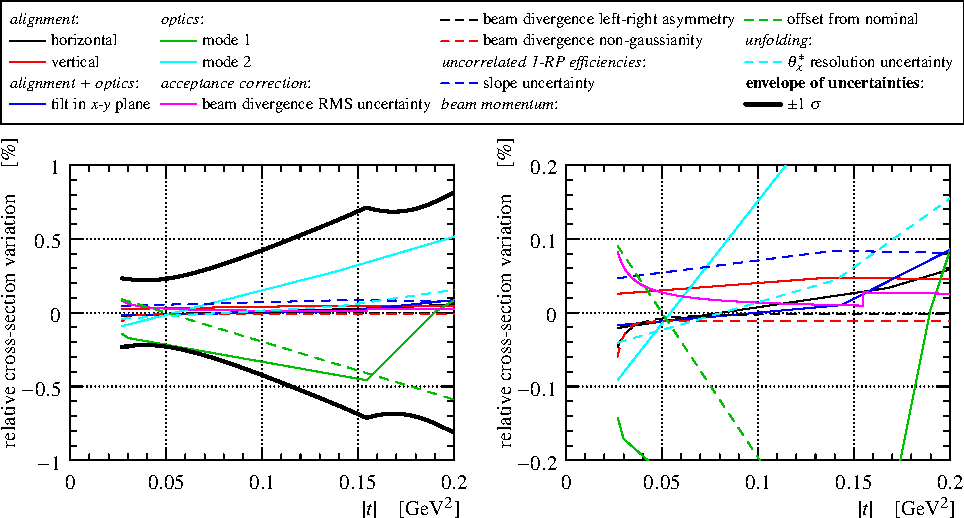
\includegraphics{fig/direct_method_mode_cmp_presentation.pdf}
\vskip-3mm
\caption{%
Impact of systematic effects on the differential cross-section. Each curve corresponds to a systematic error at $1\un{\sigma}$, cf.~Eq.~(\ref{eq:syst mode}).
The two contributions due to optics correspond to the two vectors in Eq.~(\ref{eq:opt bias modes}).
The envelope is determined by summing all shown contributions in quadrature for each $|t|$ value.
}
\label{fig:syst unc}
\end{center}
\end{figure*}

Eventually, the differential cross-section histograms from both diagonals are merged. This is accomplished by a per-bin weighted average, with the weight given by inverse squared statistical uncertainty. The statistical and systematic uncertainties are propagated accordingly. For the systematic ones, the correlation between the diagonals is taken into account. For example, the vertical (mis-)alignment of the RPs within one unit is almost fully correlated, thus the effect on the differential cross-section is opposite in the two diagonals, and consequently its impact is strongly reduced once the diagonals are merged.

The final systematic uncertainties are summarised in Figure~\ref{fig:syst unc} where their impact on the differential cross-section is shown. The leading uncertainties include normalisation, optics imperfections and beam momentum offset. Their effects are quantified in Table~\ref{tab:data}, which can be used to approximate the covariance matrix of systematic uncertainties:
\begin{equation}
\label{eq:covar mat}
\mat V_{ij} = \sum_{q} \delta s_{q}(i)\, \delta s_{q}(j)\: ,
\end{equation}
where $i$ and $j$ are bin indices (row numbers in Table~\ref{tab:data}) and the sum goes over the leading error contributions $q$ (four right-most columns in the table).


\begin{table*}
\caption{%
The elastic differential cross-section as determined in this analysis using the ``optimised'' binning. The three left-most columns describe the bins in $t$. The representative point gives the $t$ value suitable for fitting~\cite{lafferty94}.
%uncertainty due to different fit models negligible:$10^{-7}\un{GeV^2}$
The other columns are related to the differential cross-section. The four right-most columns give the leading systematic biases in $\d\sigma/\d t$ for $1\sigma$-shifts in the respective quantities, $\delta s_q$, see Eqs.~(\ref{eq:syst mode}) and (\ref{eq:covar mat}). The two contributions due to optics correspond to the two vectors in Eq.~(\ref{eq:opt bias modes}).
}
\vskip-2mm
\label{tab:data}
\begin{center}
\small
\setlength{\tabcolsep}{3.5pt}
\begin{tabular}{ccc@{\hskip20pt}ccccccc}
\hline
\hline
\multispan3\hss\vrule width0pt depth4pt height10pt $|t|$ bin $\unt{GeV^2}$\hss & \multispan7\hss $\d\sigma/\d t \ung{mb/GeV^2}$ \hss \cr
\multispan3\hrulefill\hbox to15pt{\hfil} & \multispan7\hrulefill \cr
left & right & representative & value & statistical     & systematic  & normalisation & optics   & optics   & beam\cr
edge & edge  & point      &       & uncertainty      & uncertainty   &  $\mathcal{N}$     & mode 1   & mode 2   & momentum\cr
\hline
$0.02697$ & $0.03005$ & $0.02850$ & $300.94\S$ & $0.612\S$ & $12.68\S$ & $+12.66\S$ & $-0.473\S$ & $-0.259\S$ & $+0.254\S$ \cr
$0.03005$ & $0.03325$ & $0.03164$ & $284.04\S$ & $0.554\S$ & $11.91\S$ & $+11.90\S$ & $-0.495\S$ & $-0.214\S$ & $+0.204\S$ \cr
$0.03325$ & $0.03658$ & $0.03491$ & $265.59\S$ & $0.506\S$ & $11.17\S$ & $+11.15\S$ & $-0.484\S$ & $-0.172\S$ & $+0.157\S$ \cr
$0.03658$ & $0.04005$ & $0.03831$ & $247.90\S$ & $0.465\S$ & $10.44\S$ & $+10.43\S$ & $-0.472\S$ & $-0.133\S$ & $+0.114\S$ \cr
$0.04005$ & $0.04365$ & $0.04184$ & $231.95\S$ & $0.430\S$ & $\S9.740$ & $+\S9.727$ & $-0.459\S$ & $-0.0968$ & $+0.0740$ \cr
$0.04365$ & $0.04740$ & $0.04551$ & $215.35\S$ & $0.398\S$ & $\S9.061$ & $+\S9.048$ & $-0.445\S$ & $-0.0638$ & $+0.0378$ \cr
$0.04740$ & $0.05129$ & $0.04933$ & $199.89\S$ & $0.369\S$ & $\S8.405$ & $+\S8.393$ & $-0.431\S$ & $-0.0338$ & $+0.0051$ \cr
$0.05129$ & $0.05534$ & $0.05330$ & $184.55\S$ & $0.342\S$ & $\S7.775$ & $+\S7.763$ & $-0.415\S$ & $-0.0069$ & $-0.0240$ \cr
$0.05534$ & $0.05956$ & $0.05743$ & $170.71\S$ & $0.318\S$ & $\S7.171$ & $+\S7.159$ & $-0.399\S$ & $+0.0170$ & $-0.0498$ \cr
$0.05956$ & $0.06394$ & $0.06173$ & $156.62\S$ & $0.295\S$ & $\S6.594$ & $+\S6.581$ & $-0.382\S$ & $+0.0380$ & $-0.0721$ \cr
$0.06394$ & $0.06850$ & $0.06620$ & $142.96\S$ & $0.274\S$ & $\S6.044$ & $+\S6.031$ & $-0.365\S$ & $+0.0561$ & $-0.0913$ \cr
$0.06850$ & $0.07324$ & $0.07085$ & $131.31\S$ & $0.254\S$ & $\S5.521$ & $+\S5.508$ & $-0.348\S$ & $+0.0715$ & $-0.107\S$ \cr
$0.07324$ & $0.07817$ & $0.07568$ & $119.59\S$ & $0.236\S$ & $\S5.027$ & $+\S5.013$ & $-0.330\S$ & $+0.0842$ & $-0.120\S$ \cr
$0.07817$ & $0.08329$ & $0.08071$ & $108.28\S$ & $0.218\S$ & $\S4.560$ & $+\S4.546$ & $-0.312\S$ & $+0.0944$ & $-0.130\S$ \cr
$0.08329$ & $0.08862$ & $0.08593$ & $\S97.732$ & $0.202\S$ & $\S4.122$ & $+\S4.107$ & $-0.293\S$ & $+0.102\S$ & $-0.138\S$ \cr
$0.08862$ & $0.09417$ & $0.09137$ & $\S87.916$ & $0.186\S$ & $\S3.711$ & $+\S3.696$ & $-0.275\S$ & $+0.108\S$ & $-0.143\S$ \cr
$0.09417$ & $0.09994$ & $0.09702$ & $\S78.866$ & $0.172\S$ & $\S3.329$ & $+\S3.313$ & $-0.257\S$ & $+0.112\S$ & $-0.145\S$ \cr
$0.09994$ & $0.10593$ & $0.10290$ & $\S70.641$ & $0.158\S$ & $\S2.973$ & $+\S2.957$ & $-0.239\S$ & $+0.113\S$ & $-0.146\S$ \cr
$0.10593$ & $0.11217$ & $0.10902$ & $\S62.480$ & $0.145\S$ & $\S2.644$ & $+\S2.628$ & $-0.221\S$ & $+0.113\S$ & $-0.145\S$ \cr
$0.11217$ & $0.11866$ & $0.11538$ & $\S55.454$ & $0.133\S$ & $\S2.341$ & $+\S2.325$ & $-0.204\S$ & $+0.112\S$ & $-0.142\S$ \cr
$0.11866$ & $0.12540$ & $0.12199$ & $\S48.733$ & $0.122\S$ & $\S2.063$ & $+\S2.047$ & $-0.187\S$ & $+0.109\S$ & $-0.138\S$ \cr
$0.12540$ & $0.13242$ & $0.12887$ & $\S42.712$ & $0.111\S$ & $\S1.810$ & $+\S1.793$ & $-0.170\S$ & $+0.106\S$ & $-0.132\S$ \cr
$0.13242$ & $0.13972$ & $0.13602$ & $\S37.277$ & $0.102\S$ & $\S1.580$ & $+\S1.563$ & $-0.155\S$ & $+0.101\S$ & $-0.126\S$ \cr
$0.13972$ & $0.14730$ & $0.14346$ & $\S32.207$ & $0.0922$ & $\S1.372$ & $+\S1.356$ & $-0.140\S$ & $+0.0961$ & $-0.118\S$ \cr
$0.14730$ & $0.15520$ & $0.15120$ & $\S27.731$ & $0.0835$ & $\S1.185$ & $+\S1.169$ & $-0.125\S$ & $+0.0911$ & $-0.110\S$ \cr
$0.15520$ & $0.16340$ & $0.15925$ & $\S23.827$ & $0.0764$ & $\S1.016$ & $+\S1.002$ & $-0.0942$ & $+0.0855$ & $-0.102\S$ \cr
$0.16340$ & $0.17194$ & $0.16761$ & $\S20.364$ & $0.0715$ & $\S0.865$ & $+\S0.854$ & $-0.0582$ & $+0.0793$ & $-0.0938$ \cr
$0.17194$ & $0.18082$ & $0.17632$ & $\S17.249$ & $0.0666$ & $\S0.733$ & $+\S0.723$ & $-0.0298$ & $+0.0729$ & $-0.0853$ \cr
$0.18082$ & $0.19005$ & $0.18537$ & $\S14.480$ & $0.0630$ & $\S0.618$ & $+\S0.609$ & $-0.0080$ & $+0.0664$ & $-0.0769$ \cr
$0.19005$ & $0.19965$ & $0.19478$ & $\S12.124$ & $0.0585$ & $\S0.517$ & $+\S0.508$ & $+0.0052$ & $+0.0598$ & $-0.0687$ \cr
\hline
\hline
\end{tabular}
\end{center}
\end{table*}

%----------------------------------------------------------------------------------------------------

\subsection{Statistical Uncertainty Adjustment}
\label{sec:stat unc adj}

The statistical fluctuations in the differential cross-section using the ``optimised'' binning have been slightly overestimated (the ``per-mille'' binning does not suffer from this problem). One way of demonstration is splitting the data into groups of consecutive points small enough for a linear function to approximate well the differential cross-section within each group. Then, performing straight-line fits through each group yields $\chi^2$ values slightly too low. Alternatively, the issue can be demonstrated as follows. The data sample is divided into several sub-samples corresponding to the same luminosity, and the analysis method described in the earlier sections is repeated for each of these sub-samples. Then, fluctuations of each bin content are determined from the several sub-samples, giving values slightly lower than the uncertainty estimates.
% Interpretation?

As a remedy, the statistical uncertainties in the ``optimised'' binning have been divided by a factor of $1.176$. This value has been determined by requiring both binnings to give the same value of $\chi^2/\hbox{ndf}$ for fits of $\d\sigma / \d t$ to the fit function in Eq.~(\ref{eq:fit param}) with $N_b = 3$ which has enough flexibility to describe the data.

% between the differential cross-section data and a function with enough flexibility (see the green fit in Figure~\ref{fig:data rel ob}).
